\section{Bubblesort}

\textbf{Bubblesort} ist ein \textbf{stabiles}, auf Schlüsselvergleichen basierendes \textbf{internes} Sortierverfahren, dass \textbf{in place} sortiert.

\subsection{Methode}
\textbf{Bubblesort} vergleicht zwei benachbarte Elemente und vertauscht diese miteinander, falls ihre relative Reihenfolge nicht der erwarteten Sortierreihenfolge entspricht.\\
Nach dem ersten Durchlauf steht der größte  Schlüssel\footnote{oder der kleinste Schlüssel, entsprechend den Anforderungen an die Sortierreihenfolge} am Ende des Feldes.\\
Dann wird der Vorgang wiederholt, es muss aber nicht mehr mit dem Schlüssel an Position $n-1$\footnote{die Anzahl der benötigten Vergleiche reduziert sich entsprechend nach jeder Iteration um mindestens $1$} verglichen werden, da dieser Schlüssel bereits seine endgültige Position in dem sortierten Feld eingenommen hat.\\
Das wird so lange wiederholt, bis keine Vertauschungen mehr aufgetreten sind oder in u.a. Implementierung das Ende der äußeren Schleife erreicht wurde.\\

\subsection{Implementierung}

\begin{minted}{java}
    boolean inversed = true;
    for (i = n - 1; i >= 0; i--) {
        inversed = false;
        for (j = 0; j < i; j++) {
            if (arr[j] > arr[j + 1]) {
                swap(arr, j, j+1);
                inversed = true;
            }
        }
        if (!inversed) {
            break;
        }
    }
\end{minted}

\subsection{Laufzeit}
Ist das Feld absteigend sortiert, wird in jeder Iteration der \code{while}-Schleife eine Fehlstellung (\textit{Inversion}) behoben (s. Abbildung~\ref{fig:inversions}).
Hierfür werden in jedem Durchlauf $n$ Schlüsselvergleiche durchgeführt.\\
Bei einer Eingabegröße von $n$ mit $\sum_{i=1}^n (n-i)$  Fehlstellungen (vgl.~\cite[87]{OW17b}) ergibt sich somit eine \textbf{Laufzeitkomplexität} von $O(n^2)$.


\begin{itemize}
    \item \textbf{Anzahl der Vergleiche und Vertauschungen}: $\frac{n * ( n - 1)}{2}$ ($O(n^2)$)
\end{itemize}


\noindent
Im günstigsten Fall muss das Feld nur einmal durchlaufen werden, um zu überprüfen, ob eine Vertauschung vorgenommen werden muss.\\


\begin{figure}
    \begin{center}
        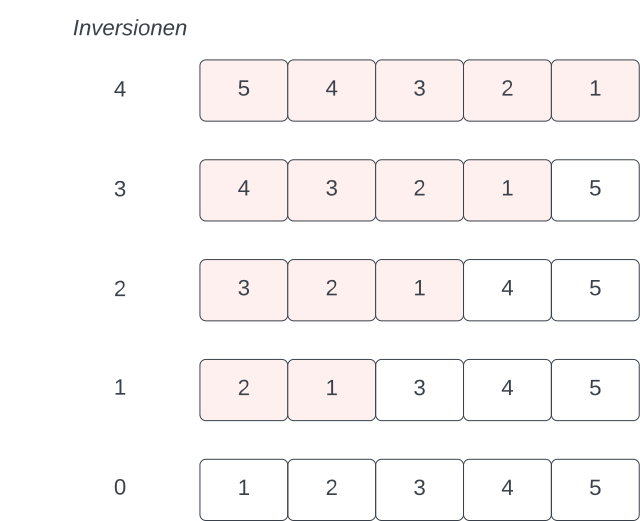
\includegraphics[scale=0.5]{chapters/Sortierverfahren/img/inversions}
        \caption{Fehlstellungen in einem absteigend sortierten Feld. (Quelle: eigene)}
        \label{fig:inversions}
    \end{center}
\end{figure}